\documentclass[12pt]{article}
\usepackage[utf8]{inputenc}

\usepackage{lmodern}

\usepackage{enumitem}
\usepackage[margin=2cm]{geometry}

\usepackage{amsmath, amsfonts, amssymb}
\usepackage{graphicx}
%\usepackage{subfigure}
\usepackage{tikz}
\usepackage{pgfplots}
\usepackage{multicol}

\usepackage{comment}
\usepackage{url}
\usepackage{calc}
\usepackage{subcaption}
\usepackage[indent=0pt]{parskip}
\usepackage{animate}

\usepackage{array}
\usepackage{blkarray,booktabs, bigstrut}
\usepackage{bigints}

\pgfplotsset{compat=1.16}

% MATH commands
\newcommand{\ga}{\left\langle}
\newcommand{\da}{\right\rangle}
\newcommand{\oa}{\left\lbrace}
\newcommand{\fa}{\right\rbrace}
\newcommand{\oc}{\left[}
\newcommand{\fc}{\right]}
\newcommand{\op}{\left(}
\newcommand{\fp}{\right)}

\newcommand{\bi}{\mathbf{i}}
\newcommand{\bj}{\mathbf{j}}
\newcommand{\bk}{\mathbf{k}}
\newcommand{\bF}{\mathbf{F}}

\newcommand{\mR}{\mathbb{R}}

\newcommand{\ra}{\rightarrow}
\newcommand{\Ra}{\Rightarrow}

\newcommand{\sech}{\mathrm{sech}\,}
\newcommand{\csch}{\mathrm{csch}\,}
\newcommand{\curl}{\mathrm{curl}\,}
\newcommand{\dive}{\mathrm{div}\,}

\newcommand{\ve}{\varepsilon}
\newcommand{\spc}{\vspace*{0.5cm}}

\DeclareMathOperator{\Ran}{Ran}
\DeclareMathOperator{\Dom}{Dom}

\newcommand{\exo}[1]{\noindent\textcolor{red}{\fbox{\textbf{Problem {#1}}}\hrulefill}\\}
\newcommand{\qu}[4]{\noindent\textcolor{#4}{\fbox{\textbf{Section {#1} | Problem {#2}}} \hrulefill{{\fbox{\textbf{{#3} Points}}}}\\}}

\newcommand{\semester}{Spring 2023}

\newcommand{\CVup}{%

\begin{tikzpicture}
\draw[black, <->, >=latex] (-0.33, 0.5) .. controls (-0.125, 0) and (0.125, 0) .. (0.33, 0.5);
\end{tikzpicture}}

\newcommand{\CVupInc}{%
\begin{tikzpicture}
\draw[black, ->, >=latex] (0,0) .. controls (0.2, 0) and (0.4, 0.2) .. (0.5, 0.5);
\end{tikzpicture}}

\newcommand{\CVupDec}{%
\begin{tikzpicture}[rotate=270]
\draw[black, ->, >=latex] (0,0) .. controls (0.2, 0) and (0.4, 0.2) .. (0.5, 0.5);
\end{tikzpicture}}

\newcommand{\CVdown}{%
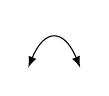
\begin{tikzpicture}
\draw[black, <->, >=latex] (-0.33, -0.5) .. controls (-0.125, 0) and (0.125, 0) .. (0.33, -0.5);
\end{tikzpicture}}

\newcommand{\CVdownInc}{%
\begin{tikzpicture}
\draw[black, ->, >=latex] (-0.5, -0.5) .. controls (-0.5, -0.3) and (-0.5, -0.1) .. (0,0);
\end{tikzpicture}}

\newcommand{\CVdownDec}{%
\begin{tikzpicture}[rotate=-90]
\draw[black, ->, >=latex] (-0.5, -0.5) .. controls (-0.5, -0.3) and (-0.5, -0.1) .. (0,0);
\end{tikzpicture}}

\begin{document}
	\noindent \hrulefill \\
	MATH-241 \hfill Pierre-Olivier Paris{\'e}\\
	Solutions Section 4-5 \hfill \semester \\\vspace*{-1cm}
	
	\noindent\hrulefill
	
	\spc	
	
	
	\exo{2}
	\\
	Let $u = 2x^2 + 3$, so that 
		\begin{align*}
		\frac{du}{dx} = 4x \quad \Ra \quad \frac{1}{4} du = x dx .
		\end{align*}
	The integral becomes
		\begin{align*}
		\int x (2x^2 + 3)^4 \, dx = \int u^4 \frac{du}{4} = \frac{u^5}{20} + C
		\end{align*}
	and the answer is
		\begin{align*}
		\frac{(2x^2 + 3)^5}{20} + C .
		\end{align*}
		
	\spc
	
	\exo{4}
	\\
	Let $u = \sin \theta$. Then
		\begin{align*}
		\frac{du}{dx} = \cos \theta \quad \Ra \quad du = \cos \theta \, dx .
		\end{align*}
	There integral becomes
		\begin{align*}
		\int \sin^2 \theta \cos \theta \, d\theta = \int u^2 \, du = \frac{u^3}{3} + C 
		\end{align*}
	and the answer is
		\begin{align*}
		\frac{\sin^3 \theta}{3} + C .
		\end{align*}
		
	\spc
	
	\exo{8}
	\\
	Let $u = x^3$, so that 
		\begin{align*}
		\frac{du}{dx} = 3x^2 \quad \Ra \quad \frac{1}{3} du = x^2 \, dx .
		\end{align*}
	Therefore, the integral becomes
		\begin{align*}
		\int x^2 \sin (x^3) \, dx = \int \sin (u) \, \frac{du}{3} = -\tfrac{1}{3} \cos (u) + C .
		\end{align*}
	The answer is then
		\begin{align*}
		-\tfrac{1}{3} \cos (x^3) + C .
		\end{align*}
		
	\spc
	
	\exo{10}
	\\
	Set $u = 1 + \cos t$, then
		\begin{align*}
		\frac{du}{dt} = -\sin (t) \quad \Ra \quad -du = \sin (t) \, dt .
		\end{align*}
	The integral then becomes
		\begin{align*}
		\int \sin t \sqrt{ 1+ \cos t} \, dt = -\int \sqrt{u} \, du = -\tfrac{2}{3} u^{3/2} + C
		\end{align*}
	and the final answer is
		\begin{align*}
		-\tfrac{2}{3} (1 + \cos t)^{3/2} + C .
		\end{align*}
		
	\spc
	
	\exo{16}
	\\
	Let $u = \sqrt{x}$, so that
		\begin{align*}
		\frac{du}{dx} = \frac{1}{2 \sqrt{x}} \, dx \quad \ra \quad 2 \, du = \frac{1}{\sqrt{x}} \, dx .
		\end{align*}
	The integral then becomes
		\begin{align*}
		\int \frac{\sin \sqrt{x}}{\sqrt{x}} \, dx = \int \sin (u) \, 2du = -2 \cos (u) + C .
		\end{align*}
	The answer is then
		\begin{align*}
		-2 \cos (\sqrt{x}) + C .
		\end{align*}
		
	\spc
	
	\exo{20}
	\\
	Let $u = x + 2$, then $du = dx$ and
		\begin{align*}
		\int x \sqrt{x + 2} \, dx = \int (u - 2) \sqrt{u} \, du = \int u^{3/2} - 2 u^{1/2} \, du = \tfrac{2}{5} u^{5/2} - \tfrac{4}{3} u^{3/2} + C .
		\end{align*}
	Then, the answer is
		\begin{align*}
		\tfrac{2}{5} (x + 2)^{5/2} - \tfrac{4}{3} (x + 2)^{3/2} + C .
		\end{align*}
	
	\spc
	
	\exo{26}
	\\
	Let $u = \tan x$, then
		\begin{align*}
		\frac{du}{dx} = \sec^2 x \, dx  .
		\end{align*}
	The integral then becomes
		\begin{align*}
		\int \frac{\sec^2 x}{\tan^2 x} \, dx = \int u^{-2} \, du = -u^{-1} + C
		\end{align*}			
	and therefore the final answer is
		\begin{align*}
		- \frac{1}{\tan x} + C .
		\end{align*}	
		
	\spc
	
	\exo{30}
	\\
	Let $u = x^2 + 1$. Therefore, we have
		\begin{align*}
		\frac{du}{dx} = 2x \quad \Ra \quad \tfrac{1}{2} du = x \, dx .
		\end{align*}	
	The integral becomes
		\begin{align*}
		\int x^3 \sqrt{x^2 + 1} \, dx = \int x^2 \sqrt{u} x \, dx = \tfrac{1}{2}\int x^2 \sqrt{u} \, du .
		\end{align*}	
	Since $u = x^2 + 1$, we have $x^2 = u - 1$ and therefore
		\begin{align*}
		\int x^2 \sqrt{u} \, du = \int (u - 1) \sqrt{u} \, du = \int u^{3/2} - u^{1/2} \, du = \frac{1}{2} \big( \frac{2}{5} u^{5/2} - \frac{2}{3} u^{3/2} \big) + C
		\end{align*}					
	and the final answer is
		\begin{align*}
		\frac{1}{5} (x^2 + 1)^{5/2} - \frac{1}{3} (x^2 + 1)^{3/2} + C .
		\end{align*}
		
	\spc
	
	\exo{36}
	\\
	Set $u = 3t - 1$ so that $\tfrac{1}{3} du = dx$ and
		\begin{align*}
		x = 0  \rightarrow u = -1 \quad \text{ and } \quad x = 1 \rightarrow u = 2 .
		\end{align*}
	After a $u$-sub, the integral becomes
		\begin{align*}
		\int_{-1}^2 u^{50} \frac{du}{3} = \frac{1}{3} \left. \big( \frac{u^{51}}{51} \big) \right|_{-1}^2 =  \frac{2^{51} + 1}{153} .
		\end{align*}
		
	\spc
	
	\exo{38}
	\\
	Let $u = x^2$, so that $\tfrac{1}{2} du = x \, dx$. The integral then becomes
		\begin{align*}
		\int_0^{\sqrt{\pi}} x \cos (x^2 ) \, dx = \frac{1}{2} \int_0^{\pi} \cos (u) \, du = \left. \sin u \right|_0^\pi = 0 .
		\end{align*}
		
	\spc
	
	\exo{46}
	\\
	The function $f(x) = x^4 \sin x$ is an odd function since
		\begin{align*}
		f(-x) = (-x)^4 \sin (-x) = - x^4 \sin (x) = f(x) .
		\end{align*}
	We divide the integral in two
		\begin{align*}
		\int_{-\pi/3}^{\pi/3} x^4 \sin x \, dx = \int_{-\pi/3}^0 x^4 \sin x \, dx + \int_0^{\pi/3} x^4 \sin x \, dx .
		\end{align*}
	The first integral in the RHS, let $u = -x$, so that $-du = dx$ and therefore
		\begin{align*}
		\int_{-\pi/3}^0 x^4 \sin x \, dx = -\int_{\pi/3}^0 (-u)^4 \sin (-u) \, du .
		\end{align*}
	Using the property of the integral:
		\begin{align*}
		-\int_{\pi/3}^0 (-u)^4 \sin (-u) \, du = \int_{0}^{\pi/3} (-u)^4 \sin (-u) \, du .
		\end{align*}
	Since $f(-u) = -f(u)$, we get that
		\begin{align*}
		\int_0^{\pi/3} (-u)^4 \sin (-u) \, du = -\int_0^{\pi/3} u^4 \sin u \, du .
		\end{align*}
	Recall that the value of the integral does not depend on the name of the variable, therefore, we have
		\begin{align*}
		\int_0^{\pi/3} u^4 \sin u \, du = \int_0^{\pi/3} x^4 \sin x \, dx 
		\end{align*}
	and so
		\begin{align*}
		\int_{-\pi/3}^{\pi/3} x^4 \sin (x) \, dx = -\int_0^{\pi/3} x^4 \sin x \, dx + \int_0^{\pi/3} x^4 \sin x \, dx = 0 .
		\end{align*}
		
\end{document}